\section{Sensorbegriff}
\begin{frame}
    \frametitle{\insertsection}
    \vfill
    \begin{definition}[Sensorelement]
        \raggedright
        Umformung von physikalischer, chemischer oder biologischer Eingangsgröße in \emph{elektrisches Messsignal}.
    \end{definition}
    \vfill
    \begin{definition}[(analoger) Sensor]
        \raggedright
        Sensorelement + aktive Messchaltung zur Umsetzung in ein normiertes analoges elektrisches Messignal.
    \end{definition}
    \vfill
    \begin{definition}[(intelligenter) Sensor]
        \raggedright
        Abtastung, Quantisierung, und \emph{digitale Ausgabe des Messignals}; evlt. \emph{Korrektur der Sensoreigenschaften}.
    \end{definition}
    \vfill
\end{frame}

\begin{frame}
    \frametitle{\insertsection}
    \vfill
    \begin{figure}
        \centerline{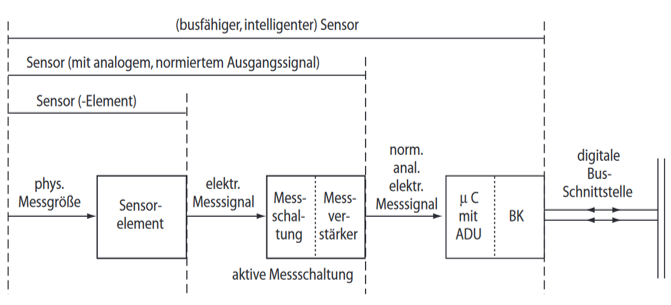
\includegraphics[height=12em]{Abbildung01_zum_sensorbegriff.png}}
        \caption{Zum Sensorbegriff[Trankler,2014]}
        \end{figure}
    \centering
    \textbf{Sensorelement: Messung \emph{nichtelektrischer} Größen.}
\end{frame}

\section{Sensoren: Einige Allgemeine Punkte}
\begin{frame}
\frametitle{\insertsection}   
\vfill
\begin{columns}
    \begin{column}[c]{0.5\textwidth}
        \begin{itemize}
            \item Sensor ist Schnittstelle zwischen Prozess und Auswertelektronik
            \begin{itemize}
                \item Direkte oder indirekte Messung
                \item Idealerweise nur selektiv für zu messende Größe und spezifisch\\
            \end{itemize}
            \item Nichtideales Verhalten
            \begin{itemize}
                \item Linearität
                \item Alterung/ Drift
                \item Quersensitivitäten\\
            \end{itemize}
            \item Unterschiedliches Ansprechverhalten
            \begin{itemize}
                \item Proportionalwertdarstellung
                \item Schwellwertschalter
            \end{itemize}
        \end{itemize}
       
    \end{column}
    \begin{column}[c]{0.5\textwidth}
        \begin{figure}
            \centerline{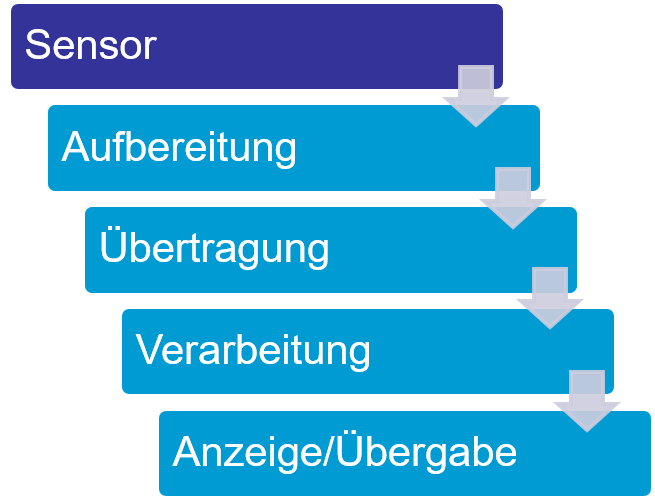
\includegraphics[height=10em]{Abbildung02.png}}
        \end{figure}
    \end{column}
\end{columns}
\end{frame}

|\section{Sensoren: Linearität und Empfindlichkeit}
\begin{frame}
    \frametitle{\insertsection}
    \vfill
    \begin{columns}
        \begin{column}[c]{0.6\textwidth}
            \textbf{Ideale Sensorkennlinie}
            \begin{equation*}
                y(x) = y_0 + \frac{\delta y}{\delta x}(x - x_0)
            \end{equation*}

            \begin{itemize}
                \item Eingangsgröße $x$
                \item Ausgangsgröße $y$
                \item $\Delta x$ Messbereich
                \item $\Delta y$ Ausgangsspanne
                \item $x_0$ Messbereichsanfang
                \item $y_0$ Ausgangssignal bei $x_0$ \\  
            \end{itemize}
            \textbf{Empfindlichkeit} (allgemein): $\varepsilon =\frac{d y}{d x}$ \\ 
            %\vspace{<len>}
            \textbf{Empfindlichkeit für linearen Sensor}:\\
             $\varepsilon =  \frac{d y}{d x}=\frac{\Delta  y}{\Delta  x} =const.$\\
        \end{column} 

        \begin{column}[c]{0.6\textwidth}
            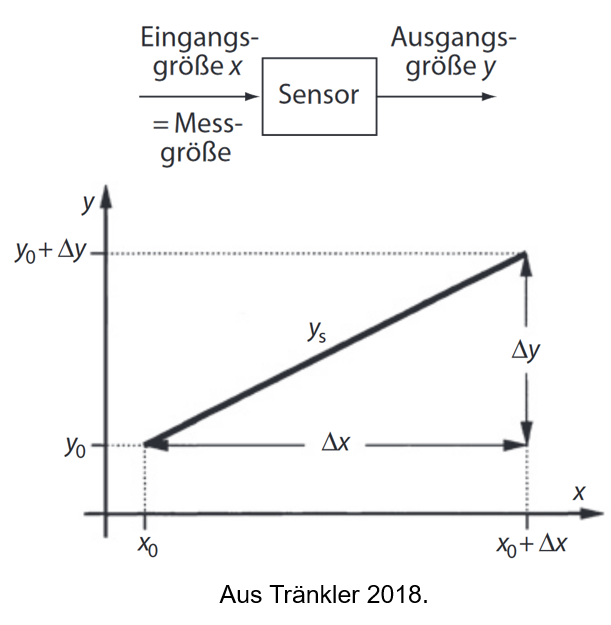
\includegraphics[height=6cm]{Abbildung03} 
        \end{column}
           
         
    \end{columns}
    
\end{frame}